\chapter{GNN \& GCN}
Molti dati del mondo reale non seguono strutture regolari in questi casi, i grafi offrono una rappresentazione più adatta: strutture composte da nodi (gli elementi) e archi (le connessioni tra essi), in grado di modellare relazioni complesse come quelle presenti nei social network, nelle molecole, nei testi, nelle immagini, nei sistemi biologici e in quelli di raccomandazione. Questo capitolo è dedicato al Graph Machine Learning, ovvero all'applicazione del Deep Learning ai dati rappresentati come grafi. Analizzeremo le Graph Neural Networks (GNN) e le principali famiglie di modelli, i problemi che possono risolvere e le tecniche per rappresentare e manipolare i dati strutturati all’interno di una rete neurale, e ci soffermeremo sulle Graph Convolutional Networks (GCN). Approfondiremo poi modelli più recenti e avanzati, come le Graph Attention Networks (GAT), GraphSAGE e le Graph Isomorphism Networks (GIN). L’obiettivo è fornire una base teorica e pratica solida per comprendere come applicare il Deep Learning anche su dati complessi come quelli rappresentati dai grafi, aprendo la strada a nuove soluzioni per problemi reali.

\section{Grafi}

Un \textbf{grafo} è una struttura flessibile in grado di rappresentare informazioni interconnesse. È composto da elementi chiamati \textit{Nodi}, connessi tra loro mediante \textit{Archi} (o \textit{Spigoli}). A differenza di una lista o di una sequenza, un grafo non presenta un inizio o una fine ben definiti, ed è quindi ideale per descrivere dati complessi che non seguono un ordine lineare. Gli archi possono essere unidirezionali o bidirezionali, determinando la distinzione tra grafi orientati e non orientati.
\begin{figure}
    \centering
    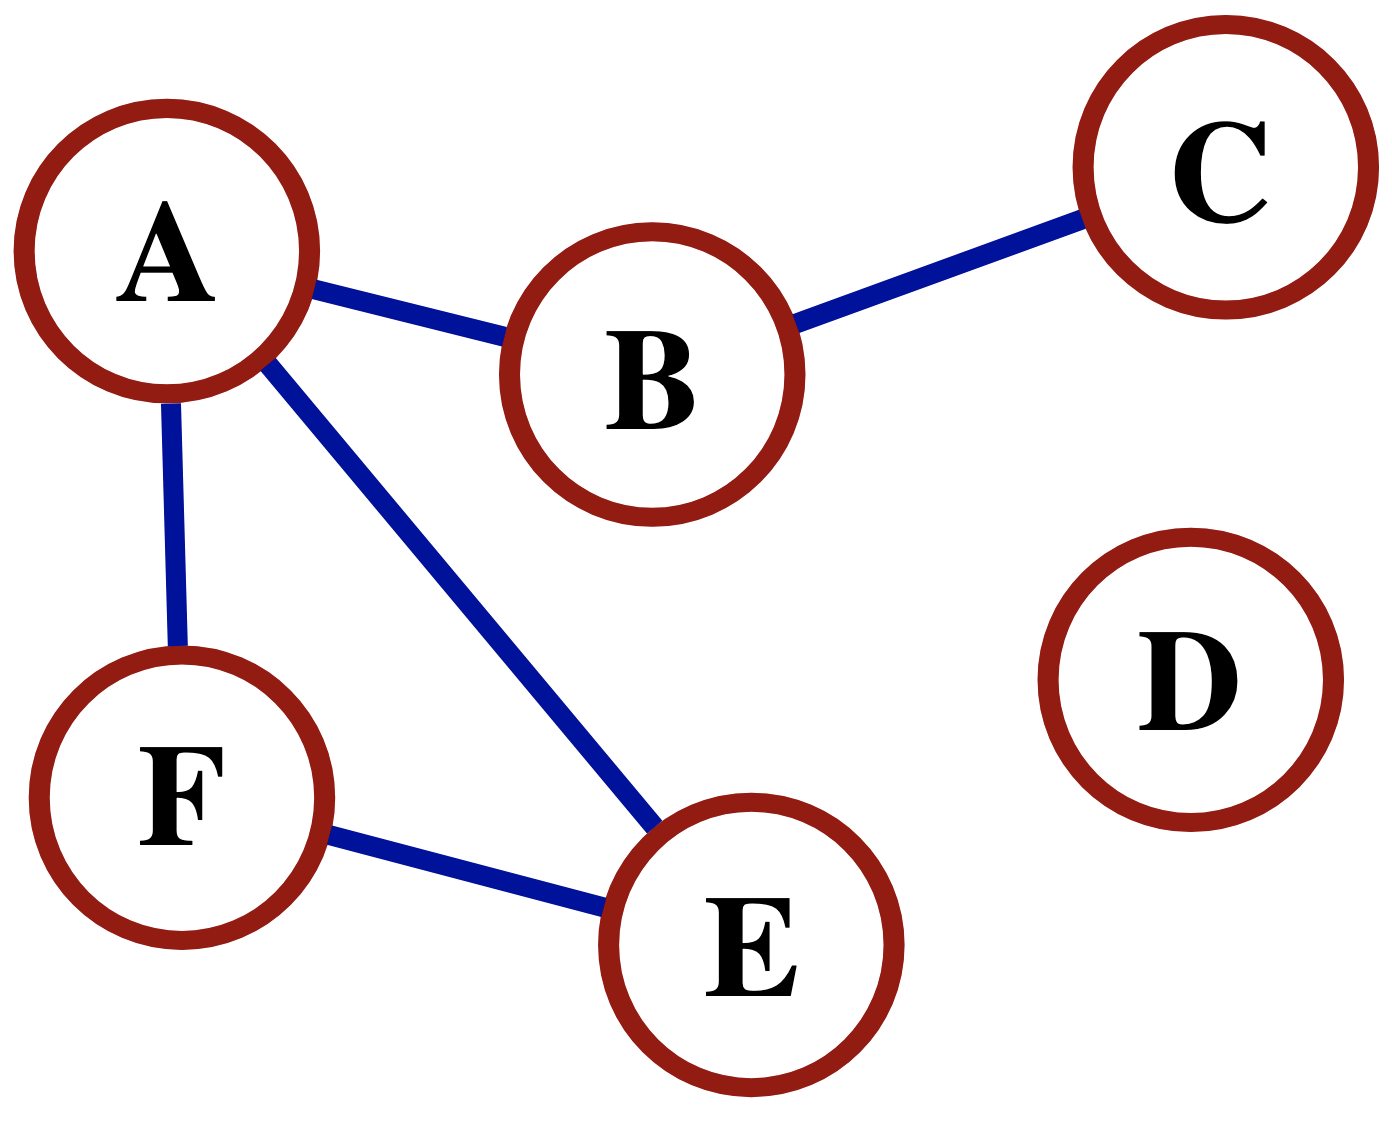
\includegraphics[width=0.4\textwidth]{figure/Graph.png}
    \caption{Esempio di grafo non orientato composto da 6 nodi e 5 archi. Se fosse orientato, gli archi avrebbero delle frecce che ne indicherebbero la direzione.}
    \label{fig:enter-label}
\end{figure}
Ogni componente del grafo può possedere attributi, i nodi possono essere caratterizzati dalla loro identità o dal numero di connessioni (\textit{grado}), gli archi invece avere un \textit{peso} che quantifica la forza della connessione. Talvolta, si introduce anche un \textit{Nodo Centrale} (o \textit{Master Node}) che sintetizza informazioni globali sul grafo.

\subsection{Immagini come grafi}

Le immagini possono essere descritte anche tramite grafi a struttura regolare. Ogni pixel corrisponde a un nodo, collegato ai pixel adiacenti, un pixel interno ha otto vicini: sopra, sotto, destra, sinistra e lungo le diagonali. L'informazione contenuta in ciascun nodo è il vettore RGB (rosso, verde, blu) del pixel. Per rappresentare le connessioni tra i nodi si utilizza la \textbf{Matrice di Adiacenza}, una struttura che indica quali nodi sono connessi, facilitando così le operazioni computazionali sul grafo.

\begin{figure}
    \centering
    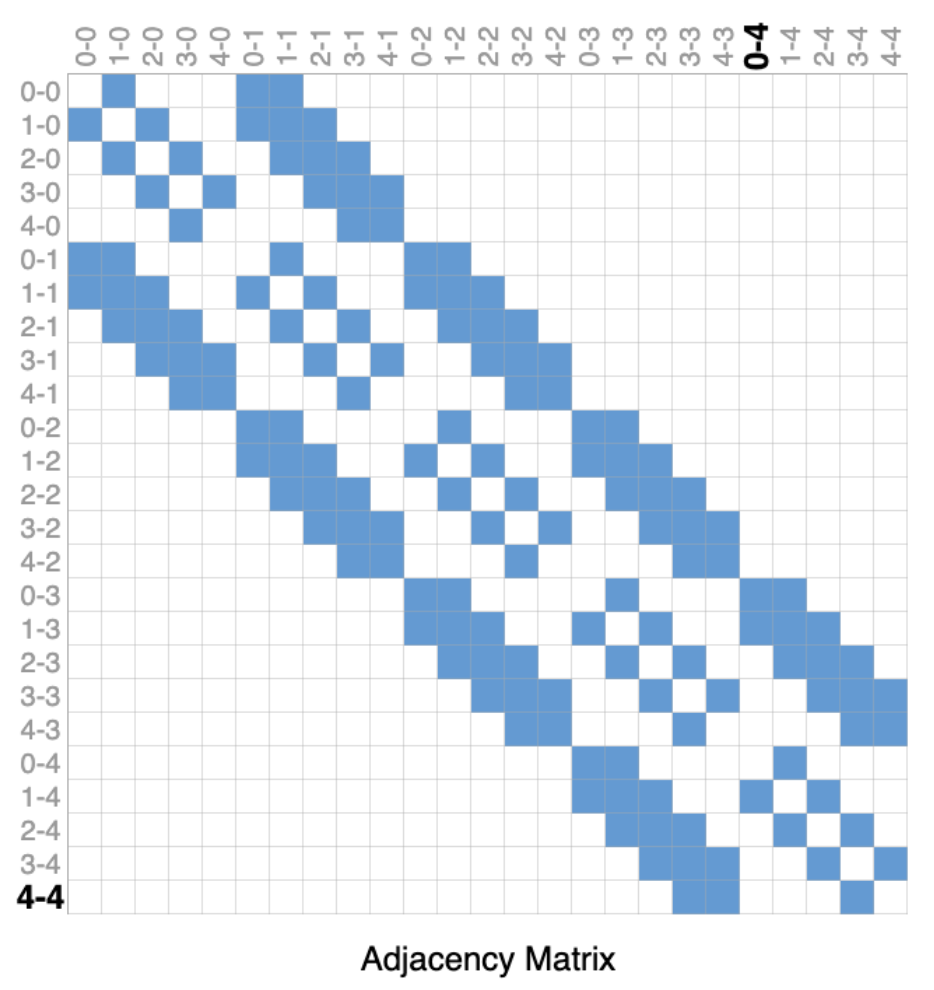
\includegraphics[width=0.5\textwidth]{figure/AdjacencyMatrix}
    \caption{Matrice di adiacenza per un'immagine $5\times5$ raffigurante una faccina sorridente. I nodi (pixel) sono connessi se condividono un lato.}
    \label{fig:adjMatrix}
\end{figure}

\subsection{Testi come grafi}

Modellare testi e immagini come grafi, è possibile, ma non comune in quanto questi dati possiedono strutture regolari. Nei testi, ogni parola è connessa solo a quella precedente e a quella successiva, producendo matrici di adiacenza fortemente strutturate, spesso con una diagonale che riflette questa linearità.
\begin{figure}
    \centering
    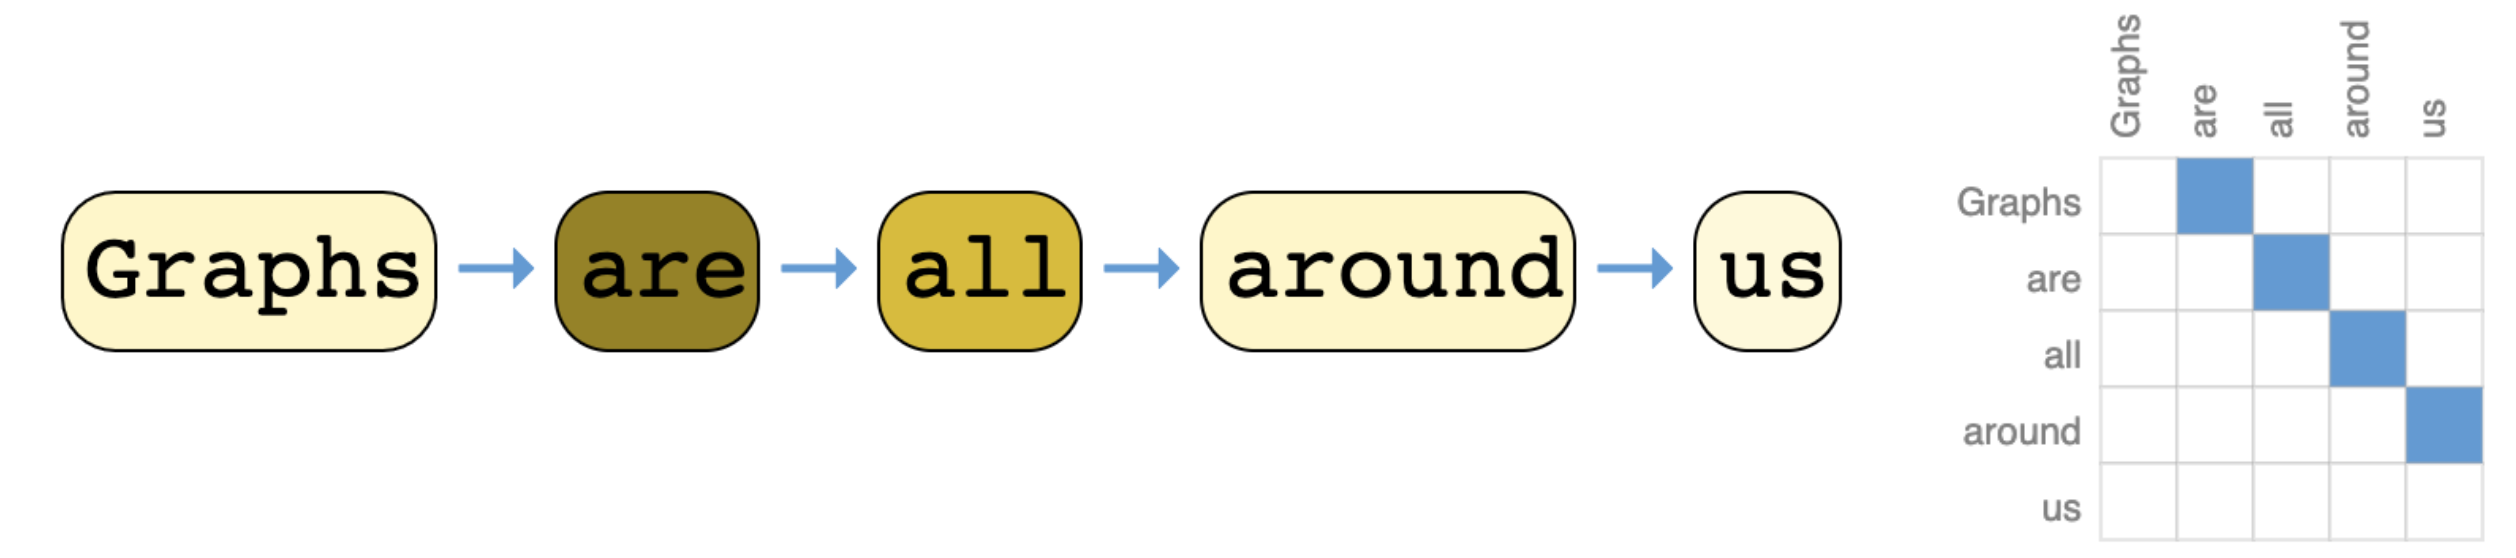
\includegraphics[width=\textwidth]{figure/TextGraph.png}
    \caption{Matrice di adiacenza di un testo: ogni parola è connessa alla precedente e alla successiva, dando origine a una struttura diagonale.}
    \label{fig:textGraph}
\end{figure}
L’uso dei grafi diventa veramente vantaggioso quando ci si confronta con dati irregolari e relazioni complesse non lineari.

\subsection{Graph-level task}

In un \textbf{Graph-level task}, l’obiettivo è predire una proprietà che riguarda l’intero grafo. L’analisi di molecole è un esempio: modellandole come grafi, si può cercare di predire l’odore, la tossicità, o il recettore con cui si legheranno. Questo tipo di task è analogo a quello della classificazione di immagini, in cui si assegna un’etichetta all’intera immagine, ma possiamo trovare anche nel NLP un parallelo: la \textit{Sentiment Analysis}, che determina il tono emotivo di un intero testo.

\subsection{Node-level task}

Nei \textbf{Node-level task}, l’obiettivo è classificare ciascun nodo individualmente. Un esempio classico è il \textit{Zachary’s Karate Club}, un dataset che rappresenta un social network diviso in due fazioni a seguito di un conflitto tra due leader. Il compito consiste nel prevedere a quale fazione appartiene ciascun membro.
\begin{figure}
    \centering
    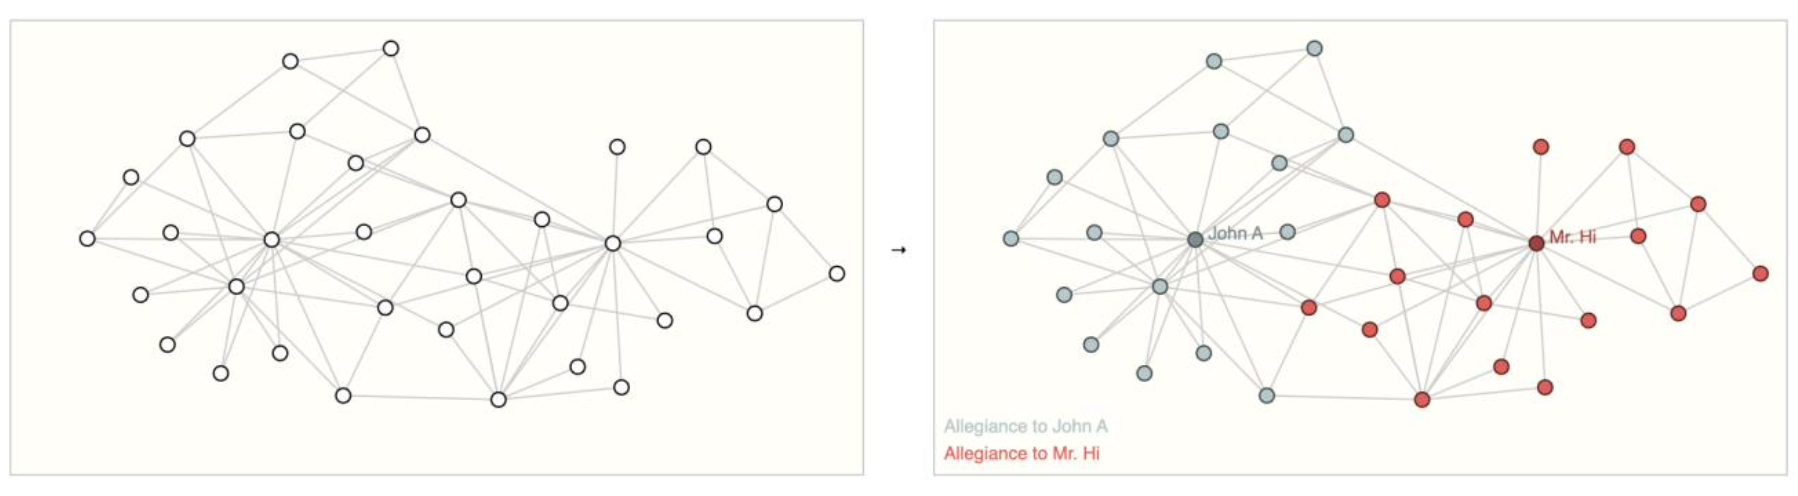
\includegraphics[width=\textwidth]{figure/ZachsKarateClubProblem.png}
    \caption{Zachary’s Karate Club: a sinistra, la rete prima della divisione; a destra, i due gruppi dopo lo scisma.}
    \label{fig:ZKCProblem}
\end{figure}
Questo problema è analogo alla segmentazione nelle immagini, in cui ogni pixel viene etichettato, mentre nel NLP, un compito simile è il \textit{part-of-speech tagging}, dove si assegna a ogni parola una categoria grammaticale.

\subsection{Edge-level task}

Un'altra tipologia di problema è l’\textbf{Edge-level task}, esso riguarda la previsione delle relazioni tra coppie di nodi. Come nella comprensione di scene: una rete neurale può essere impiegata non solo per identificare oggetti, ma anche per determinare le relazioni tra essi. In questi compiti si costruisce spesso un grafo completamente connesso, per esplorare il maggior numero possibile di interazioni tra nodi e migliorare la comprensione complessiva della struttura.

\section{Computazione sui grafi}

I grafi sono modelli flessibili, questa flessibilità però implica l’assenza di una struttura fissa. Nel compito di prevedere la tossicità di una molecola in base alla sua struttura, le molecole in esame possono variare per numero e tipo di atomi, nonché per le caratteristiche dei legami chimici. Rendere questi grafi computabili richiede quindi una rappresentazione adatta al compito. Quando si usano grafi, una semplice permutazione dei nodi, può produrre matrici di adiacenza diverse pur partendo dallo stesso grafo. Questo rende evidente che non esiste un’unica rappresentazione definibile corretta, il modello dunque deve essere progettato per essere invariante a queste permutazioni.

\subsection{Ordine dei nodi}

Convertire un grafo in un vettore richiede l'ordinamento dei nodi, ma lo stesso grafo può essere rappresentato in più modi equivalenti. Per questo motivo, un buon algoritmo deve essere \textbf{invariante rispetto all’ordine dei nodi}: qualsiasi permutazione non dovrebbe alterare l’output.
\begin{figure}
    \centering
    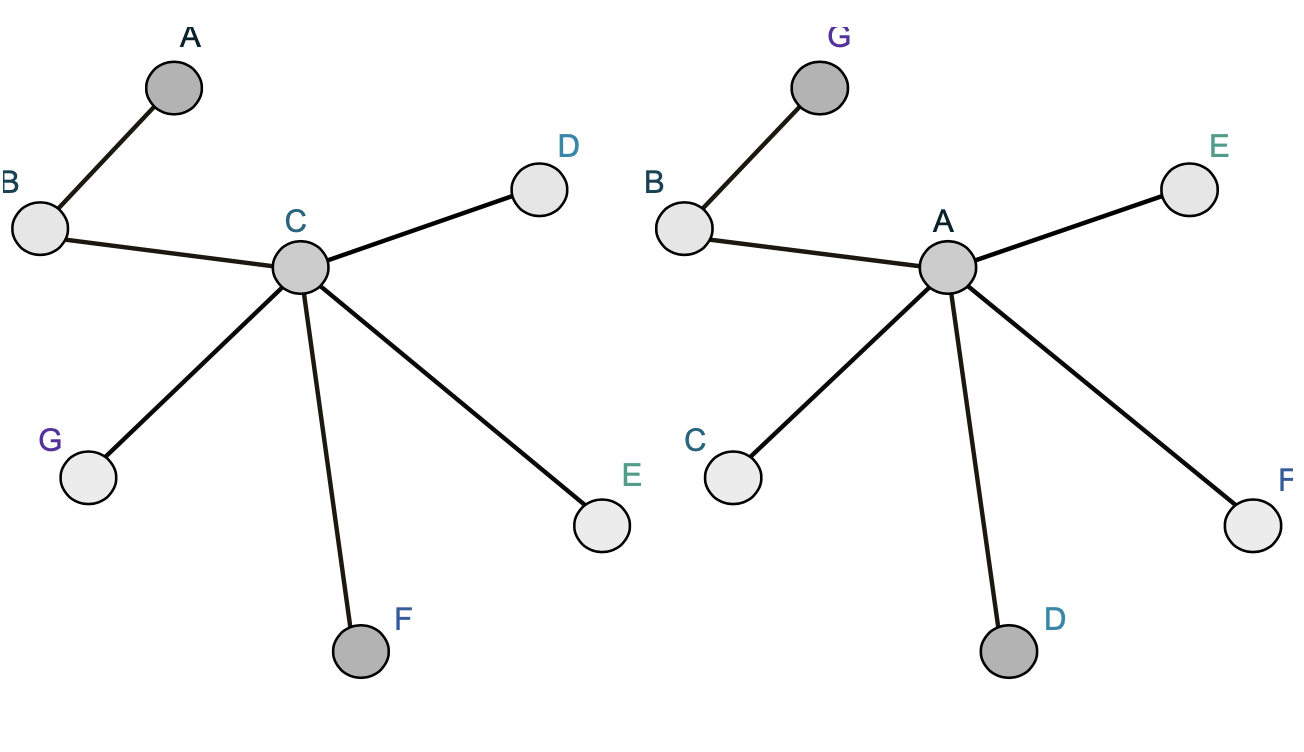
\includegraphics[width=0.7\textwidth]{figure/OrderNode}
    \caption{Due rappresentazioni diverse di un alfabeto attraverso un grafo. Sebbene l’ordine dei nodi sia differente, il significato sottostante è identico.}
    \label{fig:ordNode}
\end{figure}

\subsection{Scalabilità}

I grafi possono raggiungere dimensioni notevoli, come accade ai grafi rappresentativi dei social network i quali contano oltre un miliardo di utenti. In questi casi, ogni nodo può avere attributi complessi, e l’insieme delle connessioni, forma strutture molto ampie. Fortunatamente, i grafi reali tendono a essere \textit{sparsi}, cioè ogni nodo è connesso solo a una piccola porzione degli altri facilitando la loro rappresentazione.

\subsection{Rappresentazione dei grafi}

I grafi possono essere rappresentati in diverse modalità, una delle più efficienti è la lista di adiacenza (Figura~\ref{fig:GraphComp}). La connettività tra i nodi viene descritta tramite delle tuple, ciascuna posta nella posizione corrispondente al nodo sorgente all'interno della lista. Consentendo di evitare la computazione e la memorizzazione di porzioni disconnesse del grafo, ipotizzando che il numero di archi sia inferiore al quadrato del numero di nodi (cioè, che la matrice di adiacenza sia sparsa). È importante sottolineare che la rappresentazione in figura, utilizza valori scalari per gli attributi dei nodi, degli archi e del contesto globale, ma nella pratica i modelli GNN operano generalmente con vettori di caratteristiche. Pertanto, anziché avere un tensore dei nodi di dimensione $[n \operatorname{nodes}]$, avremo un tensore di forma $[n \operatorname{nodes}]$, $[\operatorname{node dim}]$, analogamente per archi e attributi globali.

\begin{figure}
    \centering
    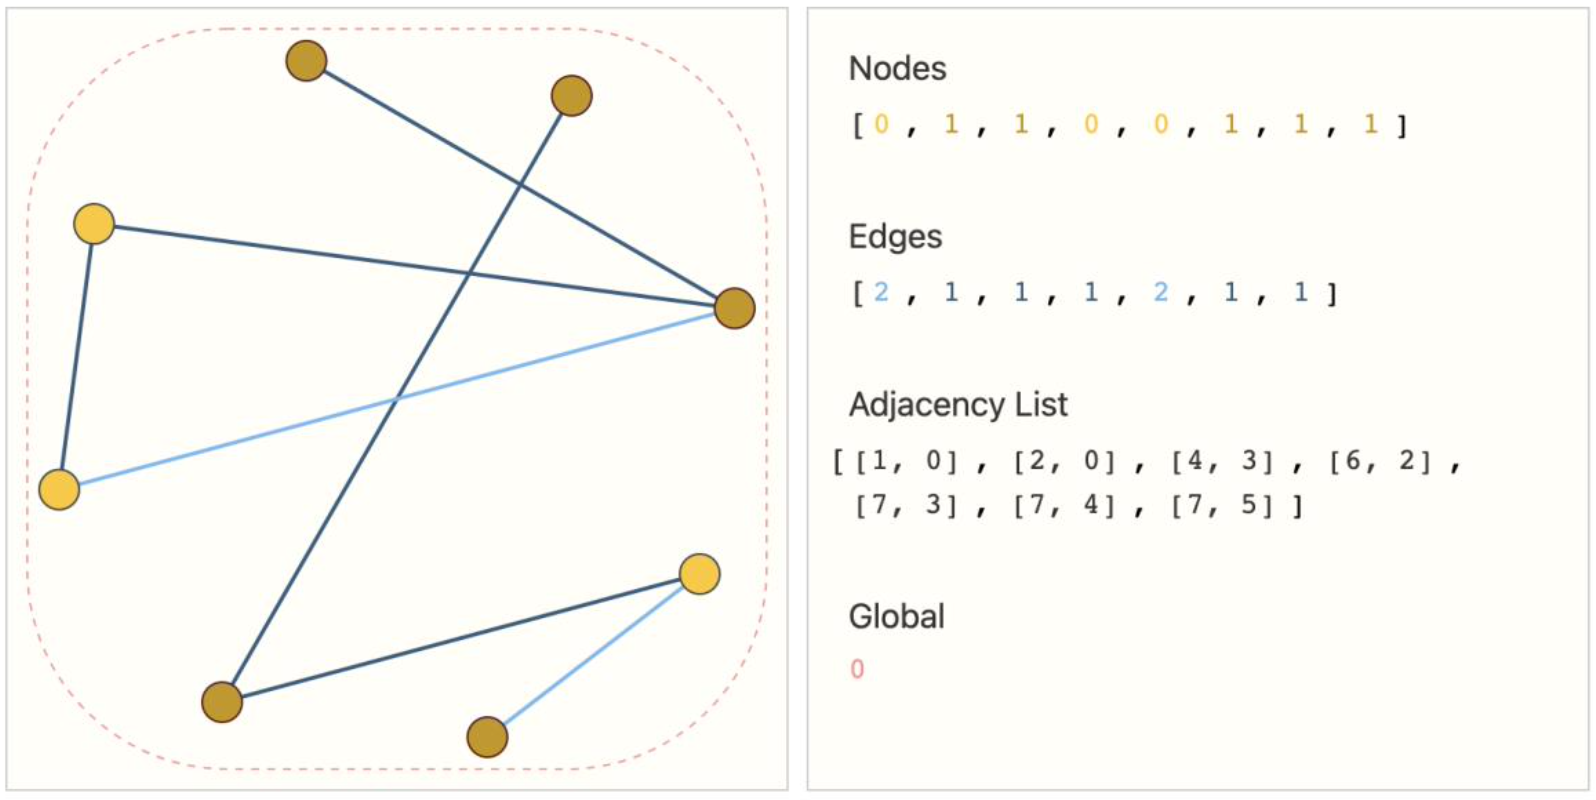
\includegraphics[width=\textwidth]{figure/ComputGraph.png}
    \caption{Rappresentazione attraverso una lista di adiacenza per un grafo computazionale.}
    \label{fig:GraphComp}
\end{figure}

\section{Graph Neural Network}

Le \textbf{Graph Neural Network} (GNN) sono modelli progettati per apprendere rappresentazioni su strutture a grafo. Una GNN è una trasformazione che agisce su tutti gli attributi del grafo, mantenendo invariata la sua struttura topologica (cioè la connettività tra nodi). Nel seguito, descriveremo le GNN seguendo il framework delle Message Passing Neural Network (MPNN), introdotto da Gilmer et al. (2017)~\cite{gilmer2017neural}, e implementato secondo lo schema delle Graph Nets proposte da Battaglia et al. (2018)~\cite{battaglia2018relational}. Questi modelli adottano una filosofia Graph-in, Graph-out: prendono in input un grafo con attributi associati a nodi, archi e contesto globale, e restituiscono un grafo trasformato, con la stessa struttura ma con rappresentazioni (embedding) aggiornate.

\subsection{La GNN più semplice}

Analiziamo l’architettura GNN più semplice, in questa configurazione, il modello apprende nuovi embedding per ogni componente del grafo, senza sfruttare le relazioni topologiche tra i nodi, cioè senza considerare la connettività. Questa GNN elementare applica un Multilayer Perceptron (MLP) separato a ciascun tipo di elemento del grafo. In particolare, a ogni nodo viene applicata una MLP che restituisce un nuovo embedding; lo stesso avviene per ogni arco e per il vettore del contesto globale. Questo layer viene comunemente definito GNN layer.

\subsection{Pooling delle informazioni}

Il termine pooling nelle GNN fa riferimento all’operazione di aggregazione delle informazioni provenienti da più elementi del grafo, con lo scopo di costruire una rappresentazione compatta dell’intero grafo o di una sua porzione. Questo è particolarmente utile nei compiti di classificazione o regressione a livello di grafo o di sotto-grafo. Nel nostro caso, consideriamo un problema di classificazione binaria a livello di nodo: se i nodi contengono già informazioni sufficienti, è possibile applicare direttamente una classificazione lineare agli embedding appresi. Tuttavia, non sempre è disponibile un'informazione utile nei nodi, in queste situazioni è necessario inferire tali informazioni aggregandole dagli archi adiacenti (Figura~\ref{fig:aggEdg}).
\begin{figure}
    \centering
    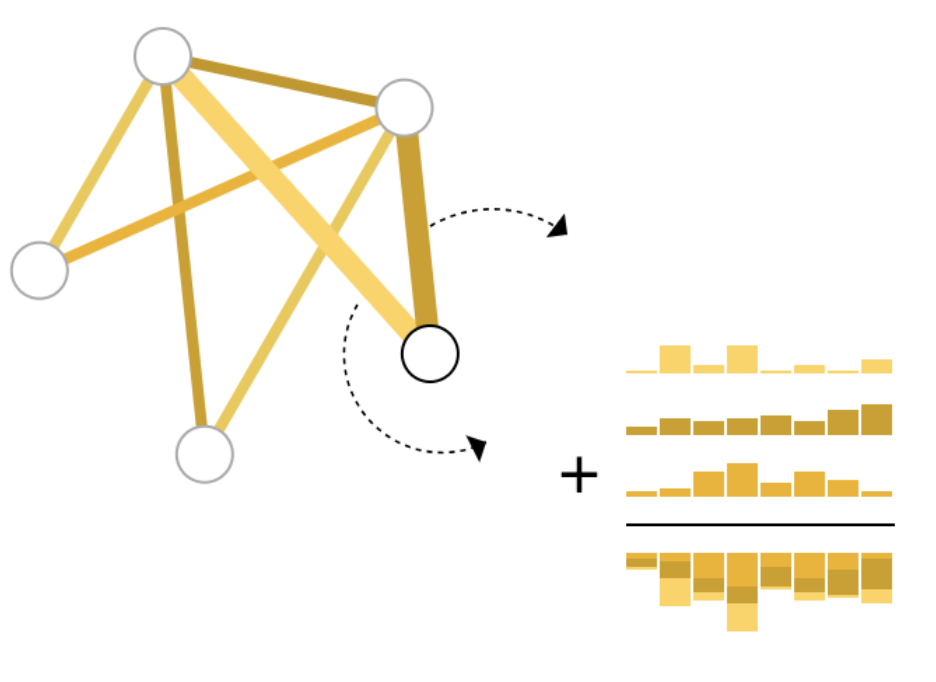
\includegraphics[width=0.8\textwidth]{figure/AggEdges.png}
    \caption{In assenza di informazioni nei nodi, è possibile inferirle aggregando quelle presenti negli archi adiacenti.}
    \label{fig:aggEdg}
\end{figure}
Il processo di pooling può essere formalizzato in due fasi principali:

\begin{enumerate}
    \item Per ciascun elemento da aggregare, si raccolgono gli embedding degli elementi correlati, e li si organizza in una matrice;
    \item La matrice ottenuta viene aggregata tramite una funzione, tipicamente una somma o una media, per ottenere un singolo embedding rappresentativo.
\end{enumerate}

Questo approccio è una strategia generica che consente di dedurre informazioni mancanti in: un nodo, un arco o nel contesto globale. Permettendoci di aggregare gli embedding degli elementi circostanti.

\subsection{Message Passing}

L’aggregazione delle informazioni è stata eseguita indipendentemente dalla connettività del grafo, una strategia ben più potente consiste nell’integrare la topologia del grafo nel processo di apprendimento. Questo è possibile grazie alla tecnica del Message Passing, gli elementi del grafo scambiano informazioni con i loro vicini, aggiornando i rispettivi embedding in base alla struttura del grafo. Questo meccanismo si articola in tre fasi:

\begin{enumerate}
    \item Per ogni nodo, si raccolgono gli embedding dei nodi adiacenti (e, se necessario, degli archi connessi);
    \item Le informazioni raccolte vengono aggregate tramite una funzione (ad esempio, una somma o una media);
    \item Il risultato dell’aggregazione viene passato a una funzione di aggiornamento (generalmente un MLP) per produrre un nuovo embedding per il nodo.
\end{enumerate}

\begin{figure}
    \centering
    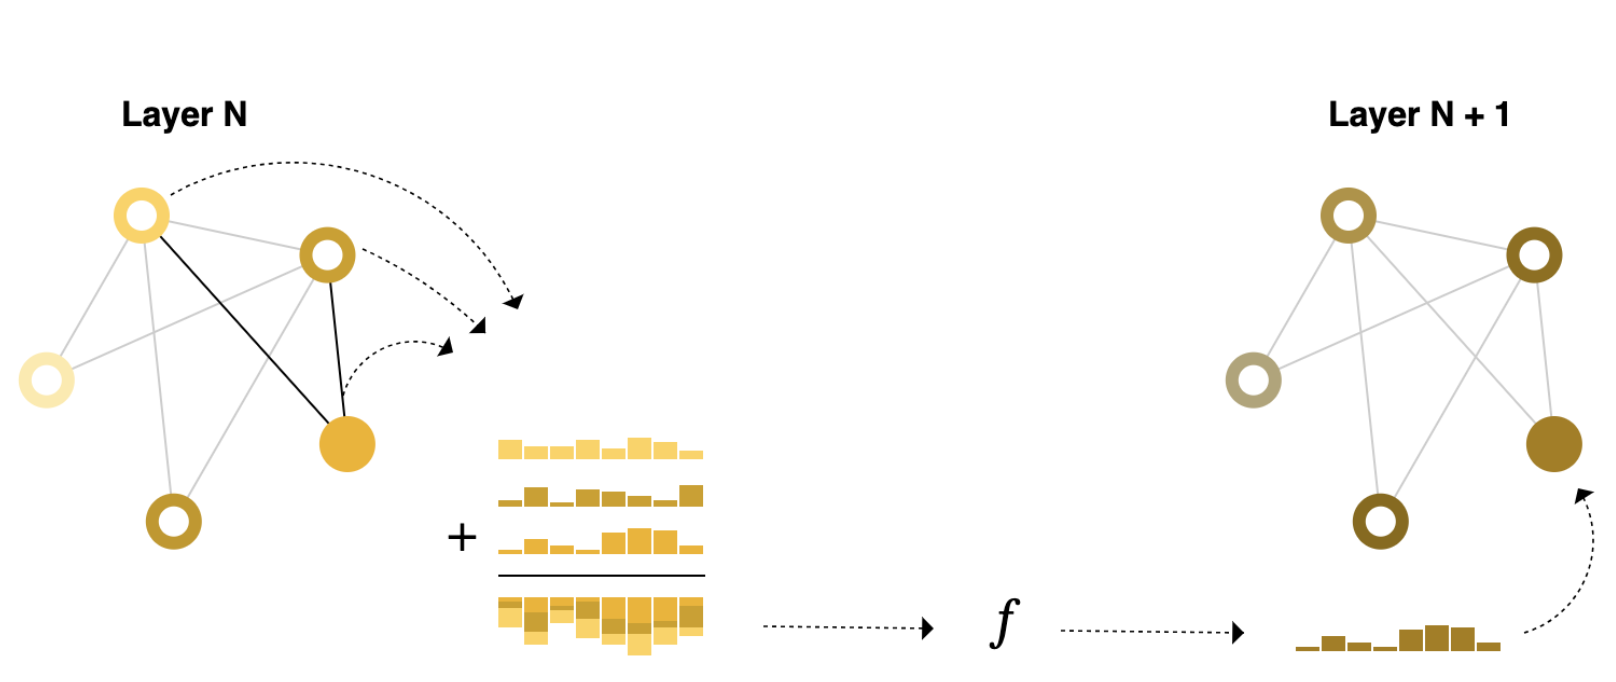
\includegraphics[width=\textwidth]{figure/MessagePassing.png}
    \caption{Fasi della Message Passing: aggregazione dei nodi adiacenti, trasformazione tramite MLP, aggiornamento degli embedding.}
    \label{fig:messPass}
\end{figure}
Questo processo può essere applicato non solo ai nodi, ma anche agli archi. La grande differenza rispetto ai pixel in un’immagine, è che i nodi possono trasmettere e ricevere informazioni anche da nodi lontani, potenzialmente aggregando conoscenza da tutto il grafo. Un ulteriore miglioramento consiste nel condividere informazioni già durante il processo di message passing, anziché solo al termine. Combinare direttamente embedding di nodi e archi può non essere immediato, poiché questi vettori possono avere dimensioni diverse. Una soluzione comune è apprendere mappature lineari tra lo spazio degli archi e quello dei nodi (e viceversa). La scelta della sequenza e del tipo di aggiornamenti rappresenta un'importante decisione di progettazione dell'architettura GNN.

\subsection{Rappresentazione globale}

Una delle limitazioni delle reti descritte finora risiede nella difficoltà di trasferire efficacemente informazioni tra nodi molto distanti all’interno del grafo. Applicando la tecnica del message passing in maniera ripetuta, non sempre le informazioni si propagano efficientemente. Una soluzione è quella di fornire a ciascun nodo una \textbf{rappresentazione globale}, solitamente indicata con $U$, nota anche come \textbf{Master Node}. Questo contesto globale è connesso a tutti i nodi e archi del grafo, e agisce come un canale condiviso per lo scambio di informazioni tra le componenti del grafo. Tale approccio consente di costruire una rappresentazione più ricca e articolata dell’intero grafo, che può essere appresa durante l’addestramento.

\subsubsection{Conditioning}

Un metodo efficace per arricchire l'embedding di un nodo è il \textbf{Conditionig}, esso prevede l'integrazione delle informazioni locali con quelle provenienti dai nodi e dagli archi adiacenti, oltre al contesto globale. Questa tecnica porta alla costruzione di rappresentazioni più informative e robuste (Figura~\ref{fig:condit}).

\begin{figure}
    \centering
    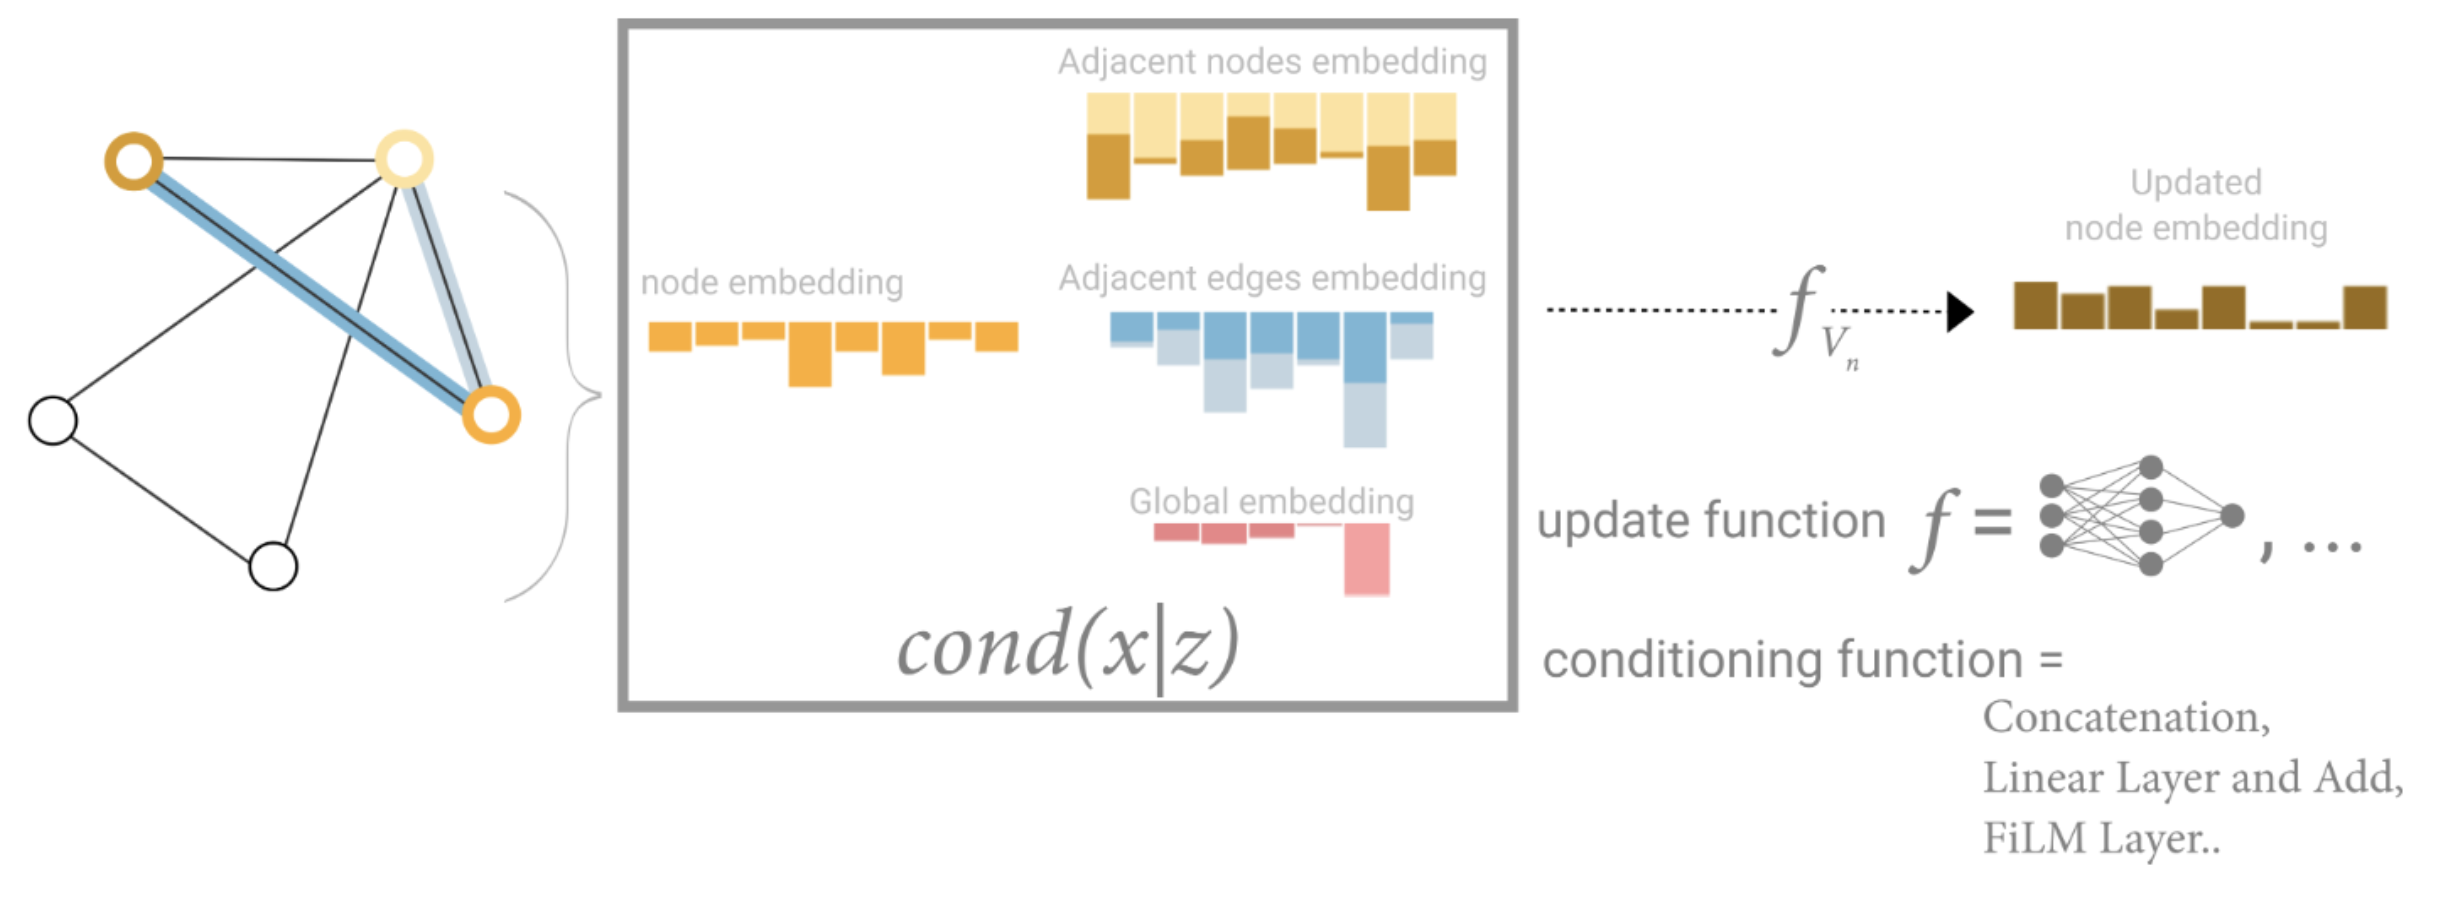
\includegraphics[width=\textwidth]{figure/Conditioning.png}
    \caption{Rappresentazione del Conditioning applicato all'embedding di un nodo, arricchito mediante gli embedding dei nodi e degli archi adiacenti, e quello relativo al contesto globale.}
    \label{fig:condit}
\end{figure}

\subsection{Filtri polinomiali sui grafi}

Nelle Graph Neural Networks (GNN), i \textit{filtri polinomiali} rappresentano uno strumento chiave per estendere il concetto di convoluzione ai dati strutturati sotto forma di grafo. Nelle immagini, la convoluzione è un’operazione locale che combina i pixel vicini in base a un kernel. Nei grafi, invece, non abbiamo una griglia regolare, ogni nodo può avere un numero diverso di vicini. Per estendere il concetto di “filtro locale”, si usa il Laplaciano del grafo: un operatore che descrive come ogni nodo è collegato agli altri. In questa sezione ne descriviamo la formulazione, l’interpretazione e i vantaggi.

\subsubsection{Il Laplaciano del grafo}

Dato un grafo \( G = (V, E) \) con matrice di adiacenza \( A \), dove \(A_{ij}\) ha valore unitario, qual'ora i nodi i e j sono connessi, la \textbf{matrice dei gradi} \( D \) è definita come:
\[
  D_{ii} = \sum_{j} A_{ij}
\]
Il \textbf{Laplaciano non normalizzato} del grafo è dato da:
\[
  L = D - A
\]

Questo operatore misura "quanto un nodo differisce dalla media dei suoi vicini", una versione alternativa è il \textbf{Laplaciano normalizzato}:
\[
  \mathcal{L} = I - D^{-1/2} A D^{-1/2}
\]
Questo serve a rendere il contributo di ciascun nodo indipendente dal suo grado (cioè dal numero di connessioni). Tale operatore discreto è l’analogo del Laplaciano continuo impiegato in analisi matematica e fisica. Definito \( L \), è possibile costruire polinomi in \( L \):
\[
  p_w(L) = \sum_{k=0}^d w_k L^k
\]
dove:
\begin{itemize}
  \item \( w_k \) sono coefficienti, i parametri appresi dal modello;
  \item \( d \) è il grado del polinomio, che controlla quanto lontano guardiamo.
\end{itemize}
Applicare l’operazione \( p_w(L) x \) consente di propagare le feature \( x \in \mathbb{R}^n \), dunque le informazioni, tra nodi del grafo.

\subsubsection{Interpretazione: Convoluzione Locale}
Nel dominio delle immagini, la convoluzione è una media pesata dei pixel vicini. Sul grafo, $L^k$ ha un effetto simile: collega ogni nodo con i suoi vicini a distanza $k$.
\begin{itemize}
  \item \( L^0 x = x \): il nodo vede solo se stesso;
  \item \( Lx \): il nodo riceve informazioni solo dai suoi vicini diretti;
  \item \( L^2 x \): il nodo integra le informazioni anche dai vicini dei vicini.
\end{itemize}
Quindi, il filtro $p_w(L)$ agisce come un kernel convoluzionale con raggio $d$, dove $d$ controlla la "profondità di diffusione" nel grafo.

\subsubsection{Esempio: Filtro di grado 1}
Il caso più semplice è proprio il Filtro di grado 1:
\[
  p_w(L) = w_0 I + w_1 L
\]
Applicandolo a un vettore \( x \), otteniamo:
\[
  x' = w_0 x + w_1 Lx
\]
Quindi il primo termine, manterrà le feature originali del nodo, mentre il secondo termine aggiungerà informazioni dai nodi adiacenti. Questo è esattamente ciò che avviene nella Graph Convolutional Network (GCN)~\cite{kipf2017semi}: ogni nodo aggiorna la propria rappresentazione combinando sé stesso e i suoi vicini in modo pesato.

\subsubsection{Intuizione finale}
I filtri polinomiali rappresentano il modo "spettrale" di fare convoluzione nei grafi:

\begin{itemize}
    \item Si basano sull’eigen-decomposition del Laplaciano, cioè sulla "frequenza" delle connessioni nel grafo;
    \item Il polinomio $p_w(L)$ agisce come un filtro passa-basso, che attenua il rumore strutturale e favorisce la propagazione tra nodi collegati;
    \item Quando $d$ è basso, la propagazione è locale (pochi hop);
    \item Aumentando $d$, il filtro diventa più globale, ma può portare al problema dell’oversmoothing (i nodi diventano troppo simili tra loro).
\end{itemize}

\subsection{Chebyshev Polynomials (ChebNet)}
Abbiamo visto che nei filtri polinomiali sui grafi, la convoluzione si realizza approssimando la funzione del Laplaciano $L$ con un polinomio, il problema è che calcolare $L^k$ può risultare computazionalmente costoso e numericamente instabile. Per risolvere questa problematica Michaël Defferrard et al.~\cite{defferrard2016convolutional} introducono i polinomi di Chebyshev, base ortogonale che consente di definire filtri stabili e più efficienti sul grafo. I \textbf{Polinomi di Chebyshev} sono una famiglia di polinomi ortogonali definiti nel dominio $[-1,1]$, e hanno una forma ricorsiva molto semplice:
\[
\begin{aligned}
  T_0(x) &= 1 \\
  T_1(x) &= x \\
  T_{k+1}(x) &= 2x T_k(x) - T_{k-1}(x)
\end{aligned}
\]
Questa ricorsione è molto efficiente da calcolare e si presta perfettamente per costruire filtri che dipendono dal Laplaciano del grafo. Il filtro convoluzionale in ChebNet è definito come:
\[
  x' = \sum_{k=0}^K w_k T_k(\tilde{L}) x
\]
dove:

\begin{itemize}
    \item $w_k \rightarrow$ Parametri appresi dal filtro (uno per ogni ordine del polinomio);
    \item $T_k(L) \rightarrow$ Rappresenta la propagazione dell’informazione a distanza $k$;
    \item $\tilde{L} = \frac{2L}{\lambda_{\text{max}}(L)} - I \rightarrow$ È il Laplaciano scalato e traslato per far sì che i suoi autovalori stiano nel dominio $[-1,1]$, condizione necessaria per applicare in modo stabile i polinomi di Chebyshev.
\end{itemize}
In pratica, i \textbf{Chebyshev polynomials} offrono un modo per calcolare convoluzioni spettrali senza dover calcolare esplicitamente gli autovettori del Laplaciano, che è un’operazione costosissima $O(n^3)$.

\subsubsection{Interpretazione}

Ogni termine $Tk(\tilde{L})x$ raccoglie informazioni dai nodi a distanza $k$, in modo simile a un filtro $L^kx$, ma in maniera più stabile e bilanciata grazie alla forma ortogonale dei polinomi. Il filtro risultante è una combinazione pesata di informazioni a diversi "gradi di vicinanza" nel grafo. Si tratta quindi di una convoluzione spettrale approssimata, più efficiente delle prime formulazioni teoriche di GCN.
\subsubsection{Vantaggi dei polinomi di Chebyshev}

\begin{itemize}
  \item \textbf{Stabilità numerica:} Poiché i polinomi sono definiti su $[-1,1]$, le operazioni non esplodono né si degradano;
  \item \textbf{Efficienza:} Grazie alla ricorsione $T_{k+1}(L)=2LT_k(L)-T_{k-1}(L)$, non servono moltiplicazioni di matrici ripetute;
  \item \textbf{Località:} La convoluzione è "locale": $T_k(L)x$ dipende solo dai nodi entro $k-\operatorname{hop}$, come un kernel di dimensione limitata;
  \item \textbf{Permutational Equivariance:} L’output cambia coerentemente se si permutano i nodi del grafo (una proprietà desiderabile nelle GNN).
\end{itemize}

\subsubsection{Stacking e Non-linearità}

Analogamente alle CNN, i filtri possono essere:
\begin{itemize}
  \item Si possono impilare più strati ChebNet, ognuno che apprende una combinazione diversa di hop;
  \item Tra gli strati si applicano funzioni non lineari (come ReLU), che permettono di costruire rappresentazioni gerarchiche.
\end{itemize}
Quindi, una ChebNet è di fatto una rete convoluzionale sui grafi, in cui il kernel è approssimato da una somma di polinomi ortogonali. I Chebyshev polynomials sono una base matematica efficiente e stabile per costruire convoluzioni spettrali localizzate sui grafi. Hanno rappresentato il passaggio fondamentale tra i filtri teorici spettrali (costosi e globali) e le GCN pratiche (efficienti e locali).

\subsection{GNN in breve}

Una GNN esegue il processo di \textit{Message Passing} in modo iterativo tra i layer, la loro forma generale è:

\begin{enumerate}
    \item \textbf{Aggregazione:} per ogni nodo \( i \):
    \[
        m_i^{(l)} = \sum_{j\in \mathcal{N}(i)} f^{(l)}(h_j^{(l-1)}, h_i^{(l-1)}, e_{ij})
    \]
    dove \( h_j^{(l-1)} \) e \( h_i^{(l-1)} \) sono gli embedding al livello precedente, ed \( e_{ij} \) rappresenta le feature dell’arco;
    \item \textbf{Aggiornamento:}
    \[
        h_i^{(l)} = g^{(l)}(h_i^{(l-1)}, m_i^{(l)})
    \]
    dove \( g \) è una funzione appresa;
    \item \textbf{Readout:} una funzione aggrega le rappresentazioni dei nodi per ottenere quella dell’intero grafo.
\end{enumerate}

\section{Modern Graph Neural Networks}

Cosa accade se, invece di filtri polinomiali, adottiamo strategie di aggregazione alternative? È importante che l’aggregazione sia invariante all’ordine dei nodi, così da garantire robustezza strutturale. In questi modelli, la convoluzione viene vista come un processo di Message Passing iterato. Ogni nodo aggiorna la propria rappresentazione combinando la propria feature con quelle dei nodi adiacenti.

\subsection{Graph Convolutional Network (GCN)}

Una GCN segue due step fondamentali:
\begin{enumerate}
    \item \textbf{Aggregazione delle feature dai vicini:}
    \[
        h_v^{(k)} = f^{(k)}\left(W^{(k)} \cdot \frac{1}{|\mathcal{N}(v)|} \sum_{u \in \mathcal{N}(v)} h_u^{(k-1)} + B^{(k)} \cdot h_v^{(k-1)}\right)
    \]
    \item \textbf{Predizione finale:}
    \[
        \hat y_v = \operatorname{PREDICT}(h_v^{(K)})
    \]
\end{enumerate}
Dove $\mathcal{N}$ è l'insieme dei nodi vicini a quello preso in analisi, la funzione \( \operatorname{PREDICT} \) è una rete neurale addestrata congiuntamente al modello GCN. Le matrici \( W^{(k)} \) e \( B^{(k)} \) sono condivise tra i nodi e non dipendono dalla dimensione del grafo, il che rende il modello scalabile.

\subsection{GCN in breve}

La GCN è una GNN che utilizza convoluzioni su grafi, per ogni layer avviene:
\begin{enumerate}
    \item \textbf{Aggregazione normalizzata:}
    \[
        m_i^{(l)} = \sum_{j\in \mathcal{N}(i)} \frac{1}{\sqrt{d_i d_j}} h_j^{(l-1)}
    \]
    \item \textbf{Aggiornamento non lineare:}
    \[
        h_i^{(l)} = \sigma(W^{(l)} m_i^{(l)})
    \]
\end{enumerate}

\textbf{Conclusione:} GNN è un termine generico, mentre GCN è un’architettura specifica che applica convoluzioni sui grafi tramite aggregazione e trasformazioni lineari.

\subsection{Graph Attention Network (GAT)}
La \textbf{Graph Attention Network (GAT)} estende il paradigma delle GCN introducendo un meccanismo di \textbf{attenzione appresa}, che consente a ciascun nodo di pesare dinamicamente i contributi dei propri vicini durante l’aggregazione. In altre parole, ogni nodo decide "quanto ascoltare" ciascuno dei suoi vicini. L’aggiornamento delle feature di un nodo $v$ al livello $k$ è definito come:

\[
    h_v^{(k)} = f^{(k)}\left(W^{(k)} \cdot \sum_{u \in \mathcal{N}(v)\,\cup\, \{v\}} \alpha_{vu}^{(k-1)} h_u^{(k-1)}\right)
\]

Qui $h_v^{(k)}$ è la rappresentazione del nodo $v$ al layer $k$, $W^{(k)}$ è una matrice di pesi appresa, $f^{(k)}$ è una classica funzione di attivazione, e $\alpha_{vu}^{(k-1)}$ è il coefficiente di attenzione che indica quanto il nodo $v$ deve considerare il vicino $u$. Per ogni coppia di nodi connessi $(v,u)$ viene calcolato un punteggio di attenzione:
\begin{equation*}
    e_{vu}^{(k)} = a^{(k)}(W^{(k)}h_v^{(k-1)}, W^{(k)}h_u^{(k-1)})
\end{equation*}
Dove $a^{(k)}$ è una piccola rete neurale, tali punteggi vengono poi normalizzati tramite una \textbf{softmax} sui soli nodi adiacenti (definiti dalla matrice di adiacenza $A$:

\[
    \alpha_{vu}^{(k)} = \frac{\operatorname{exp}(e_{vu}^{(k)})}{\sum_{w\in\mathcal{N}(v)}\operatorname{exp}(e_{vw}^{(k)})}
\]
In questo modo, l’attenzione è calcolata solo sui vicini effettivi del grafo, poiché $A_{vu}=0$ implica che il nodo $u$ non viene considerato nell’aggregazione. Dopo $K$ layer di aggregazione, la rappresentazione finale del nodo $v$ è:
\[
    \hat y_v = \operatorname{PREDICT}(h_v^{(K)})
\]
I parametri \( f^{(k)}, W^{(k)}, a^{(k)} \) sono condivisi tra i nodi del grafo. Questo rende la GAT efficiente e scalabile.

\subsection{Graph SAGE}

\textbf{Graph SAGE} (Graph Sample and AggregatE) è un'architettura di GNN proposta per affrontare il problema della generalizzazione a nodi non visti durante il training, ovvero il cosiddetto \textit{inductive setting}. Invece di apprendere una rappresentazione per ogni nodo del grafo, Graph SAGE apprende una funzione di aggregazione che può essere applicata anche a nodi mai visti. Il principio di base è quello di aggiornare le rappresentazioni dei nodi tramite l'aggregazione delle feature dei vicini campionati:
\[
    h_v^{(k)} = \sigma\left(W^{(k)} \cdot \text{AGGREGATE}^{(k)}\left(\{h_v^{(k-1)}\} \cup \{h_u^{(k-1)}, \forall u \in \mathcal{N}(v)\}\right)\right)
\]
Dove:
\begin{itemize}
    \item \( h_v^{(k)} \) rappresenta l'embedding del nodo \( v \) al layer \( k \);
    \item \( \mathcal{N}(v) \) è l'insieme dei vicini di \( v \);
    \item \( \text{AGGREGATE}^{(k)} \) è una funzione (non parametrica o parametrica) che aggrega le rappresentazioni dei vicini;
    \item \( W^{(k)} \) è una matrice di pesi appresa;
    \item \( \sigma \) è una funzione di attivazione non lineare.
\end{itemize}

Alcune possibili scelte per la funzione di aggregazione includono:
\begin{itemize}
    \item \texttt{mean:} media delle rappresentazioni dei vicini;
    \item \texttt{pooling:} max-pooling o mean-pooling dopo un MLP;
    \item \texttt{LSTM:} aggregazione sequenziale tramite un LSTM.
\end{itemize}

L’approccio di Graph SAGE è particolarmente utile per scenari di \textit{streaming} o \textit{large-scale learning}, poiché permette di scalare a grafi di grandi dimensioni grazie al campionamento locale e al riutilizzo della stessa funzione aggregatrice.

\subsection{GIN}

La \textbf{Graph Isomorphism Network} (GIN) è un'architettura proposta con l’obiettivo di massimizzare il potere discriminante delle GNN. In particolare, GIN si basa sull’intuizione che molte architetture GNN esistenti non riescono a distinguere efficacemente tra strutture topologicamente diverse. GIN è costruita in modo da essere potente quanto il test di isomorfismo di Weisfeiler-Lehman (WL test), noto per la sua efficacia nel distinguere grafi non isomorfi. La formula di aggiornamento per un nodo \( v \) è la seguente:
\[
    h_v^{(k)} = \text{MLP}^{(k)} \left((1 + \epsilon^{(k)}) \cdot h_v^{(k-1)} + \sum_{u \in \mathcal{N}(v)} h_u^{(k-1)} \right)
\]
Dove:
\begin{itemize}
    \item \( \epsilon^{(k)} \) è un parametro (appreso o fisso) che bilancia il contributo del nodo rispetto ai suoi vicini;
    \item \( \text{MLP}^{(k)} \) è un multilayer perceptron che apprende una trasformazione non lineare;
    \item \( h_v^{(k)} \) rappresenta l’embedding del nodo al layer \( k \).
\end{itemize}

GIN evita normalizzazioni e pesi di attenzione, puntando su un'aggregazione semplice ma espressiva, dove l'intera struttura locale del nodo viene catturata sommando direttamente le rappresentazioni. È stato dimostrato empiricamente che GIN ottiene prestazioni molto competitive su compiti di classificazione di grafi e predizione sui nodi, grazie alla sua capacità di distinguere strutture complesse.

\begin{sidewaystable}[htbp]
    \centering
    \caption{Confronto tra le principali architetture di Graph Neural Networks.}
    \scriptsize
    \begin{tabular}{|l|c|c|c|c|}
    \hline
    \textbf{Caratteristica} & \textbf{GCN} & \textbf{GAT} & \textbf{GraphSAGE} & \textbf{GIN} \\
    \hline
    \textbf{Tipo Aggregazione} & Media normalizzata & Attenzione pesata & Custom (media, LSTM, pooling) & Somma + MLP \\
    \hline
    \textbf{Pesatura dei vicini} & Statica (matrice normalizzata) & Dinamica (self-attention) & Parametrica o fissa & Fissa (somma) \\
    \hline
    \textbf{Apprendimento Induttivo} & No & Parziale & Sì & No \\
    \hline
    \textbf{Espressività} & Limitata & Superiore a GCN & Dipende dall’aggregatore & Massima (WL test) \\
    \hline
    \textbf{Funzione di aggiornamento} & Lineare + ReLU & Lineare + Attenzione & MLP + Aggregazione & MLP su somma \\
    \hline
    \textbf{Parametri appresi} & W & W, Attenzione & W, Aggregatore (opz.) & MLP, $\epsilon$ \\
    \hline
    \textbf{Sensibile alla struttura del grafo} & Sì & Sì & Sì & Sì (con maggiore discriminatività) \\
    \hline
    \textbf{Scalabilità} & Buona & Limitata (per grafi molto grandi) & Alta (con campionamento) & Media \\
    \hline
    \textbf{Proprietà chiave} & Semplicità & Flessibilità & Generalizzazione & Massima capacità discriminante \\
    \hline
    \end{tabular}
\label{tab:GNN_comparison}
\end{sidewaystable}

